In this chapter, special concepts and features of the CosmoScout VR application are presented, which shape and
influence the methods and solutions to mitigate cybersickness symptoms presented in
chapter~\ref{ch:implemented-solutions}.

Additionally, situations and aspects of CosmoScout VR that have shown to provoke cybersickness in the simulation are
examined in the second section of this chapter to highlight the areas that the implemented solution are targeted at,
in order to alleviate the problems and provide a more comfortable user experience without unnecessarily limiting the
user.

\section{CosmoScout Concepts}\label{sec:cosmoscout-concepts}
\subsection{Control Scheme}\label{subsec:control-scheme}

\begin{figure}[h]
    \centering
    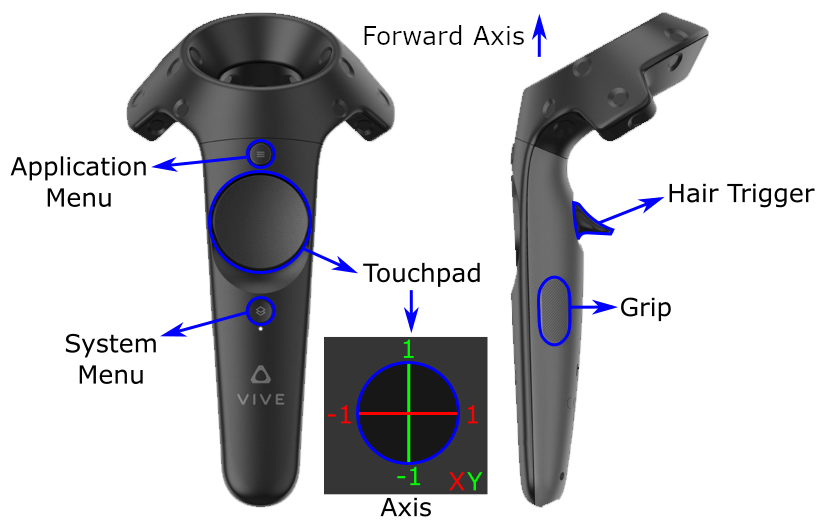
\includegraphics[width=0.6\textwidth]{content/3_current_state/img/ViveControllerButtons[BAA2017]}
    \caption{HTC Vive Remote Controller Button reference~\cite{BAA2017}.}
    \label{fig:controller-reference}
\end{figure}

The main control scheme of CosmoScout VR for HMDs employs one-handed flying controls similar to the control
scheme of Google Earth VR or the One-Hand Flying described by Drogemuller et al.~\cite{Drogemuller2020}.
The controls use the buttons highlighted in figure~\ref{fig:controller-reference}, as well as an indicator that is
drawn as an extension of the remote controller's forward pointing axis.

Pressing the touchpad allows the user to rotate the simulation around the body the user is pointing at with the
remote's indicator, i.e.\ the observer is moved around the body in circular orbits on a sphere with the radius of the
initial distance to the body.
The angle of the rotation corresponds directly to the magnitude of the vector between the initial and current position
of the indicator's intersection with the body.

Pressing the grip button allows the user to "grab" the body, the remote indicator is pointing at, and move the body
around the observers position in circular orbits on a sphere with a radius of the initial distance between the
observer and the body.
The observer is always rotated so that the "grabbed" point on the body remains at the position of the remote indicator.

Pulling the hair trigger allows the user to move the observer freely with 6 degrees of freedom (see
figure~\ref{fig:6-dof-reference}).
While the trigger is pulled, the observer's translational movement is determined by the vector from the initial
position when the trigger was pulled to the current position.
The vector's magnitude directly corresponds to the velocity of the observer in the direction of the vector.
Additionally, while the trigger is pulled, the observer's rotational movement is determined by the angles between the
initial and the current orientation of the remote.
The angles correspond to the angular velocity of the observer's rotation.
Through the translation of vector magnitude and angles of orientation into velocities, the user does not need to
twist the remote in uncomfortable positions, but can gradually navigate the simulation with small, precise movements.


\subsection{SPICE Coordinate Systems}\label{subsec:spice-coordinate-systems}

The SPICE system is provided and developed by the Navigation and Ancillary Information Facility (NAIF) of the United
States National Aeronautics and Space Administration (NASA).
The system is used to manage data sets called "kernels" and provide a precise observation geometry information 
system, originally developed to assist in planning and interpreting scientific observations from space-based 
instruments aboard robotic spacecrafts~\cite{NAIFbook, NAIFhomepage}.

SPICE is used in the CosmoScout application for precise, and time-dependent positioning of celestial objects inside
the simulation through a set of inertial and non-inertial nested reference frames.
An inertial frame is a non-rotating, and non-accelerating reference frame with respect to the surrounding stars, and
provides a static reference frame for the whole simulation.
The used inertial frame is called "J2000" and is based on the earth's equatorial plane, and the equinox, the 
intersection between the equatorial and the ecliptic plane, as described in figure~\ref{fig:J2000}.
The J2000 reference frame, is also almost coincident (rotational difference of less than $0.1$ arc seconds) with the
International Celestial Reference Frame (ICRF), which is defined by measured positions of extragalactic sources, like
quasars.

\begin{figure}[h]
    \centering
    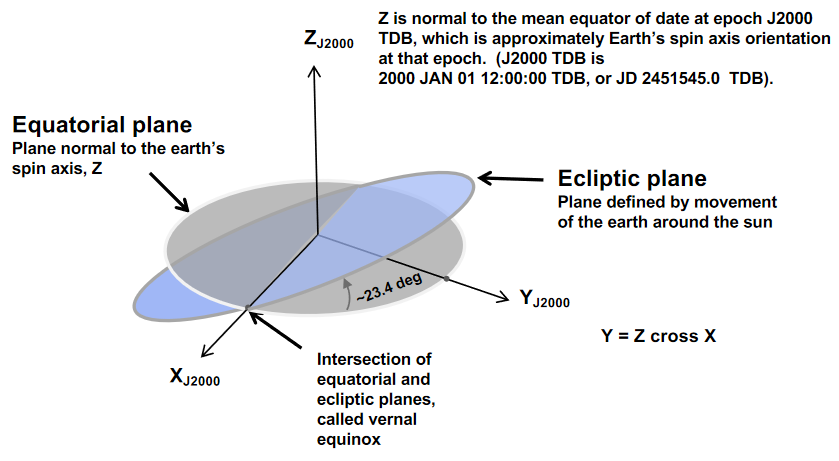
\includegraphics[width=\textwidth]{content/3_current_state/img/J2000[NAIFoverview]}
    \caption{The construction of the J2000 reference frame~\cite{NAIFoverview}.}
    \label{fig:J2000}
\end{figure}

Nested in the inertial frame are several non-inertial frames, which are accelerating frames, including rotations.
CosmoScout uses the body-fixed frames for the celestial objects in the simulation.
The center of the frame is also the center of the natural body of the frame (sun, planet, satellite, asteroid, etc.),
and the frame is tied to that body, rotating with it.
The most common named bodies have body-fixed frames hardcoded into SPICE ("IAU\_\textit{bodyname}", i.e.\ "IAU\_MARS"),
and their rotation state at any time is determined by a dataset published by the international astronomical union (IAU).

CosmoScout also uses the nested reference frames for the scene graph, to handle the large scale of the simulation, by
using frame-local scene graphs attached to the SPICE reference frame.
These, usually flat frame-local scene graphs are internally attached to the root node of the real ViSTA scene graph to
allow standard graph traversal.
This way, the observer node can be easily moved and reattached to other SPICE frames and enables easy frame
transitions during the navigation.
Additionally, the chosen reference frame for the observer is chosen automatically through a weight based on the
distance of the observer to a body, and the body's size.
The closer the observer is to a body's center, the higher the weight for the respective body-fixed reference frame.
The weight also influences the max velocity of the free navigation, and the frame in which position, and rotation, if
the weight is high enough, are tracked~\cite{SimonPaper}.

This concept is also used in section~\ref{sec:automatic-movement-overhaul}, where the term frame is used to describe
the sphere of influence, where a body's weight is dominant, resulting in the observer's position being tracked
relative to the body's reference frame.
Locations where the observer is tracked in the J2000 frame are considered interplanetary space.


\section{Identified Problems}\label{sec:identified-problems}

In order to improve usability and reduce cybersickness symptoms, we aimed to identify and improve aspects and
scenarios in CosmoScout VR that led to cybersickness symptoms or general feeling of discomfort.
To identify these problems, we conducted small tests, gathering empirical data, and used small interviews and
discussions with other developers and users of CosmoScout.
A formal study with unbiased test subjects was not done for several reasons, mainly since the goal is only vaguely
defined and may require a decently sized sample size, as well as time to process its results.
Additionally, the health and safety regulations and lockdowns around the COVID-19 outbreak complicated the feasibility
of any preliminary study.

The empirical data and interviews identified two major problem areas that need independent solutions to mitigate
discomfort and sickness symptoms.
The 6-Degrees-of-Freedom (6-DOF) in interplanetary space can easily lead to visually induced motion sickness, and the
rotations and translations of automatic navigation similarly have a tendency to lead to motion sickness symptoms,
especially the descending and ascending animations to navigate to a body's surface.


\subsection{Problems with free movement}\label{subsec:problems-with-free-movement}

While traditional 4-DOF-navigation provides an inherently more stable frame of reference with the fixed plane of
movement usually providing an up-direction strongly tied to the movement scheme, a 6-DOF-navigational system lacks this
reference frame as it allows the user to freely rotate around all axes.
A reference to the different degrees of freedom is shown in figure~\ref{fig:6-dof-reference}.

\begin{figure}[h]
    \centering
    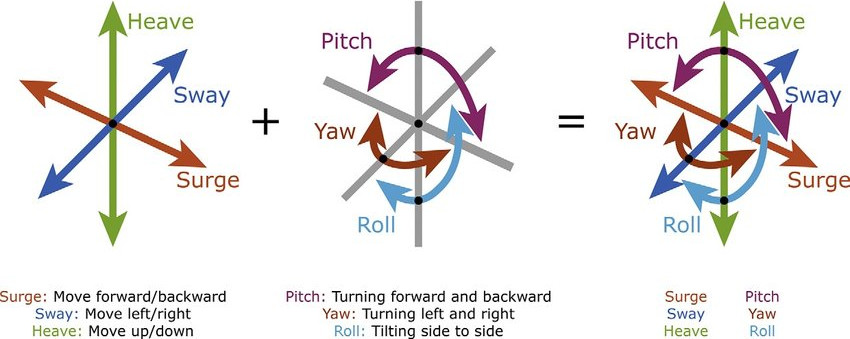
\includegraphics[width=0.6\textwidth]{content/3_current_state/img/6-DOF-reference[Fragaszy2018]}
    \caption{Six potential degrees of freedom for rotation and translation of an object~\cite{Fragaszy2018}.}
    \label{fig:6-dof-reference}
\end{figure}

Keshavarz, and Hecht~\cite{Keshavarz2011b} examined the influence of rotations around multiple axes and found that
increasingly complex rotations lead to an increase in cybersickness symptoms.
Additionally, Rebenitsch et al.~\cite{Rebenitsch2016} found multiple studies examining the effects of different
degrees of freedom in navigation.
They mention 6-DOF navigation usually induce more cybersickness symptoms than navigation with limited degrees of
freedom and conclude that the reason might be a limitation of rotation axes.
The control scheme of CosmoScout VR as described in section~\ref{subsec:control-scheme} does not allow for easy and
independent control of rotation around each axis, which can quickly lead to complex rotations around multiple axes at
once.
These complex rotations paired with a lack of reference frame can easily disorient the user and lead to visually
induced motion sickness symptoms.

While it seems both problems originate from the control scheme, a change of the control scheme does not necessarily
help mitigate the problems as different control schemes like those proposed by Drogemuller et al.~\cite{Drogemuller2020}
either suffer from the same problems, or significantly change the interaction context.
Isolating the rotation controls would be hard to implement with only the VR remotes and lead to a more unintuitive
and inconvenient control scheme.
Therefore, other mitigation methods are sought to provide the user with a stable frame of reference and reduce the
impact of complex rotations.


\subsection{Problems with automatic movement}\label{subsec:problems-with-automatic-movement}

The current automatic navigation to selected bodies or bookmarked locations was only designed as a rudimentary method
to facilitate the means of quick and precise movements to points of interest without the need for manual travel to
said point of interest.

\begin{figure}[h]
    \centering
    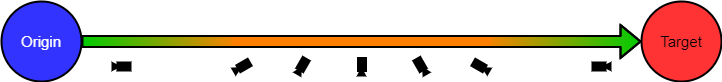
\includegraphics[width=\textwidth]{content/3_current_state/img/OldAutomaticNavigation}
    \caption{Current automatic movement between two points of interest.}
    \label{fig:old-auto-nav}
\end{figure}

The navigation uses linear interpolation between the current position and rotation, and the target position and
rotation to change both variables over a predetermined duration.
Additionally, the animation speed is variable to start the movement slow, speeding up in the intermediate travel,
before slowing down again, settling into the final position and orientation.
Figure~\ref{fig:old-auto-nav} describes the movement process between two points of interest during the automatic
navigation.
The color gradient represents the velocity of the observer in the simulation during their linear movement.
The camera icons represent the rotation of the observers field of view, and the frequency of the icons roughly
represent the angular velocity of the rotation.

Obviously, a complex rotation paired with linear movement can easily provoke visually induced motion sickness in
users experiencing these movements, as these motions resemble provocative simulations used in several studies to
actively induce cybersickness in their subjects.


\begin{wrapfigure}{o}{0.25\textwidth}
    \centering
    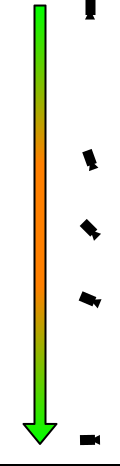
\includegraphics[width=0.1\textwidth]{content/3_current_state/img/OldAutomaticNavigation_Landing}
    \caption{Current automatic movement descending onto a body's surface.}
    \label{fig:old-auto-nav-descend}
\end{wrapfigure}

The movements to ascend or descend between a body's orbit and its surface have been mentioned by some users to be a
significant problem of the automatic movement in CosmoScout VR and source of discomfort.
The source of increased cybersickness symptoms is thought to be the more prominent reference frame provided by the
body's surface.
As presented in figure~\ref{fig:old-auto-nav-descend}, the movements use the same interpolation as mentioned above.
However, during the intermediate period, where both linear velocity of translation and angular velocity of rotation
are highest, the perceived reference frame changes.

While the observer is positioned in a body's orbit, the user's frame of reference is oriented such that the body is
"in front" of them, i.e.\ the surface's normal being perpendicular to the perceived up-direction.
During the descending movement the body's surface normal shifts to be parallel to the up-direction without the user
vestibular system feeling angular acceleration or a shift in gravity.
Paired with the disorientation during the automatic movement this strong reference frame and change of orientation may
exasperate the resulting motion sickness symptoms, as the rotations in interplanetary space only have other bodies,
and the surrounding stars as weak points of reference to indicate the rotation.
The ascending movement suffers from the same problem, but in reverse, changing the body's surface from a reference
plane parallel to the real world surface to it being perpendicular to perceived gravity.

Finally, the current navigation does not have any collision detection or handling, which can contribute to discomfort
of users when the linear path of the navigation intersects a body, as shown in figure~\ref{fig:old-auto-nav-collision}.

\begin{figure}[h]
    \centering
    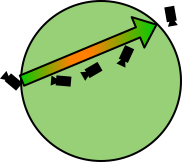
\includegraphics[width=0.25\textwidth]{content/3_current_state/img/OldAutomaticNavigation_SurfaceCollision}
    \caption{Current automatic movement between two points of interest on different sides of a body.}
    \label{fig:old-auto-nav-collision}
\end{figure}

While, collision detection and handling is not part of this study, we aimed to mitigate collision related problems in
our solutions and provide navigation methods that allows collision detection and handling to be added afterwards
without major changes to the basic structure.
